\documentclass[10pt,a4paper]{article}
\usepackage[utf8]{inputenc}
\usepackage[italian]{babel}
\usepackage{amsmath}
\usepackage{amsfonts}
\usepackage{amssymb}
\usepackage{graphicx}
\usepackage{siunitx}
\usepackage{textcomp}
\usepackage[left=2cm,right=2cm,top=2cm,bottom=2cm]{geometry}
\newcommand{\rem}[1]{[\emph{#1}]}
\newcommand{\exn}{\phantom{xxx}}
\renewcommand{\thesubsection}{\thesection.\alph{subsection}} 
\renewcommand{\thesubsubsection}{\thesection.\alph{subsection}.\alph{subsubsection}}

\title{Ottica 2: Misure interferometria}
\author{Fabrizio Chicconi, Lorenzo Cavuoti, Simone Antognetti}

\begin{document}
 \maketitle 
 
\section*{Introduzione}
 L'esperienza ha lo scopo di effettuare misure di lunghezze d'onda tramite l'interferometria ed è divisa in due parti:
 \begin{itemize}
 \item misura della lunghezza d'onda di un laser Elio-Neon tramite reticolo di diffrazione;
 \item misura della lunghezza d'onda della riga verde del mercurio tramite interferometro di Michelson.
 \end{itemize}
 
 \section*{Ottica 2A - Misura della lunghezza d'onda di un laser He-Ne}
 Lo scopo di questa parte dell'esperienza è quello di misurare la lunghezza d'onda di un laser He-Ne utilizzando un reticolo di diffrazione rappresentato dal righello graduato di un calibro. Uno schema dell'apparato sperimentale è mostrato in Fig.~\ref{fig:diff}.
 \begin{figure}[h]
 	\centering
 	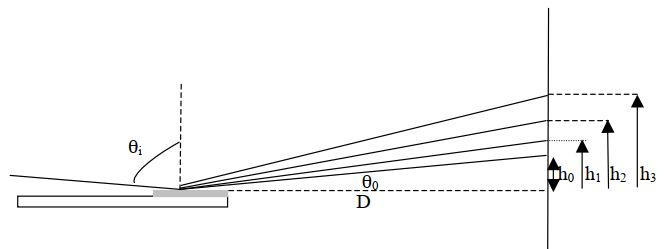
\includegraphics[scale=0.8]{calibro}
 	\caption{Schema dell'apparato sperimentale}
 	\label{fig:diff}
\end{figure}
\subsection*{Preparazione dell'apparato}
 Il passo del reticolo è di 1mm, cioè la spaziatura tra le tacche sul righello del calibro. Essendo molto grande rispetto alla lunghezza d'onda del laser che è $\sim650$ nm per poter osservare bene la diffrazione è necessario disporre il laser in modo che la luce incida in maniera quanto più possibile radente al righello, con angoli di incidenza cioè prossimi a $\pi$/2. Disponendo l'apparato come descritto sono stati osservati \rem{\dots} ordini di diffrazione.

\subsection*{Misure}
La prima misura effettuata è stata quella della distanza in orizzontale tra il punto di incidenza della luce sul calibro e lo schermo dove si formano le figure di diffrazione ottenendo D = \rem{\dots}. A questo punto si misurano le altezze a cui si osservano i vari ordini di diffrazione che sono prese a partire dal punto medio tra il punto in cui si osserva il fascio diretto sullo schermo e l'ordine zero. \newpage

\noindent Queste misure non si riportano per questione di spazio, ma in Tabella~\ref{tab:diff} sono raccolti gli angoli di diffrazione risultanti dalle relazioni:
\begin{equation*}
\mathrm{\theta_n} = \mathrm{\arctan{\frac{h_n}{D}}}
\end{equation*}
\begin{equation*}
\mathrm{\theta_{d_n}} = \frac{\pi}{2} - \mathrm{\theta_n}
\end{equation*}
dove $\mathrm{\theta_n}$ è l'angolo rispetto all'orizzontale al quale osservo l'n-esimo oridne di diffrazione sullo schermo e $\mathrm{\theta_{d_n}}$ è l'angolo di diffrazione dello stesso ordine.
\begin{table}[h]
	\centering
	\caption{Angoli di diffrazione}
	\vspace{1mm}
	\begin{tabular}{cc}
	\hline
	N° ordine & $\mathrm{\theta_{d_n}}$ \\ \hline \hline
	0 & \rem{\dots} \\
	1 & \rem{\dots} \\
	2 & \rem{\dots} \\
	3 & \rem{\dots} \\
	4 & \rem{\dots} \\
	5 & \rem{\dots} \\
	6 & \rem{\dots} \\
	7 & \rem{\dots} \\
	8 & \rem{\dots} \\
	9 & \rem{\dots} \\
	10 & \rem{\dots} \\
	11 & \rem{\dots} \\
	12 & \rem{\dots} \\
	13 & \rem{\dots} \\
	14 & \rem{\dots} \\ 
	15 & \rem{\dots} \\ \hline
	\end{tabular}
	\label{tab:diff}
\end{table}

\subsection*{Analisi dati e fit}
In questa fase si esegue l'analisi dati che porterà a stimare la lunghezza d'onda del laser He-Ne. L'equazione che si prende in considerazione è quella del reticolo:
\begin{equation*}
\mathrm{d(\sin\theta_i - \sin\theta_d) = m\lambda}
\end{equation*}
 dove d è il passo reticolare uguale ad 1mm, $\mathrm{\theta_i}$ è l'angolo di incidenza uguale all'angolo di diffrazione di ordine zero, $\mathrm{\theta_d}$ è l'angolo di diffrazione e m l'ordine. \newline
 Si riscrive la relazione ottenendo:
 \begin{equation*}
 \mathrm{\sin\theta_d} = \mathrm{-m\frac{\lambda}{d} + \sin\theta_i}.
 \end{equation*}
 Questa è l'equazione di una retta in cui l'ascissa è rappresentata da m l'ordine di rifrazione e l'ordinata da $\mathrm{\sin\theta_d}$.
 Il fit di questa retta è stato eseguito lasciando liberi i parametri $\mathrm{\lambda/d}$ e $\mathrm{\sin\theta_i}$ e sono stati ottenuti i seguenti risultati:
\begin{itemize}
\item[] $\mathrm{\lambda/d}$ = \rem{\dots} $\Rightarrow$ $\lambda$ = \rem{\dots}
\item[] $\sin\theta_i$ = \rem{\dots}
\item[] $\chi^2/\mathrm{ndof}$ = \rem{\dots}
\item[] P value = \rem{\dots}
\end{itemize} 
\newpage
\noindent In Fig.~\ref{fig:fit} sono mostrati il grafico del fit e dei residui normalizzati.
\begin{figure}[h!]
	\centering
	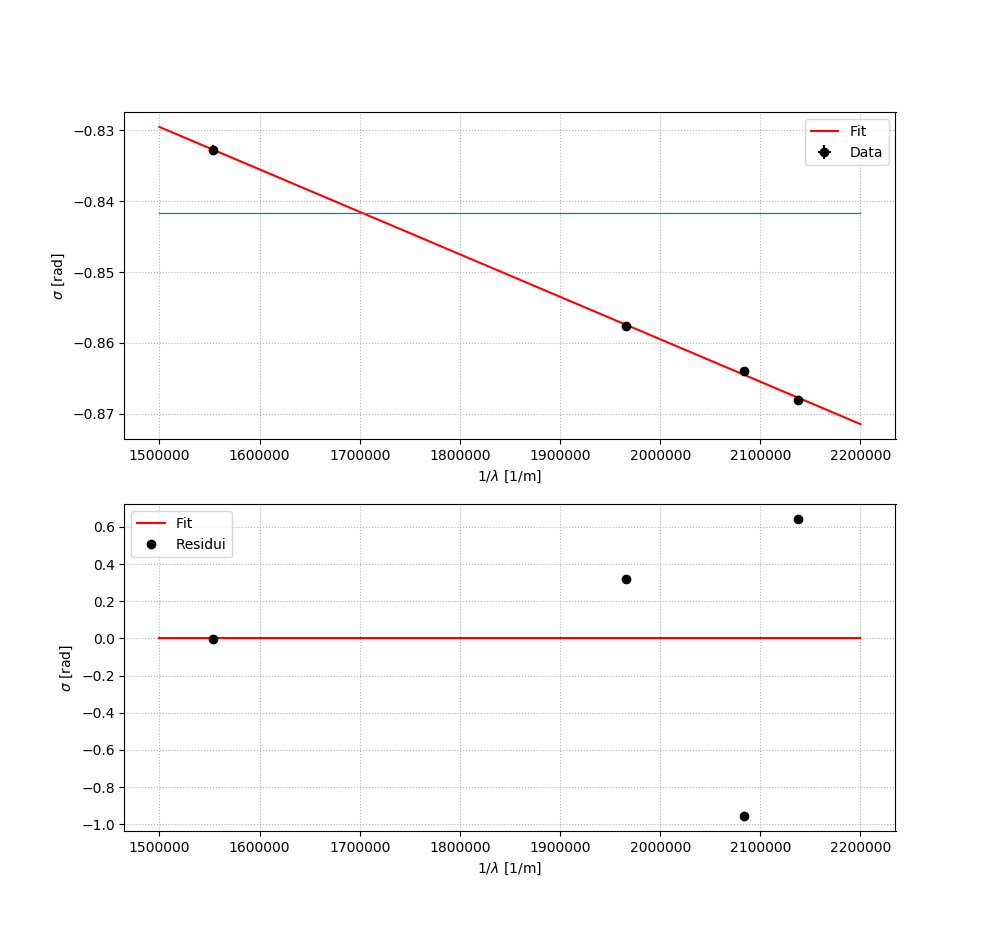
\includegraphics[scale=0.5]{fit_calibro}
	\caption{Fit e residui normalizzati}
	\label{fig:fit}
\end{figure}
\subsection*{Conclusioni}
I risultati ci permetto di concludere che \dots
\newpage
\section*{Ottica 2B - Interferometro di Michelson}
In questa parte dell'esperienza si vuole misurare la lunghezza d'onda di una lampada al mercurio utilizzando i dati ottenuti con una sorgente a lunghezza d'onda nota rappresentata dal laser ad He-Ne. L'apparato utilizzato è l'interferometro di Michelson mostrato in Fig.~\ref{fig:int}.
\begin{figure}[h]
	\centering
	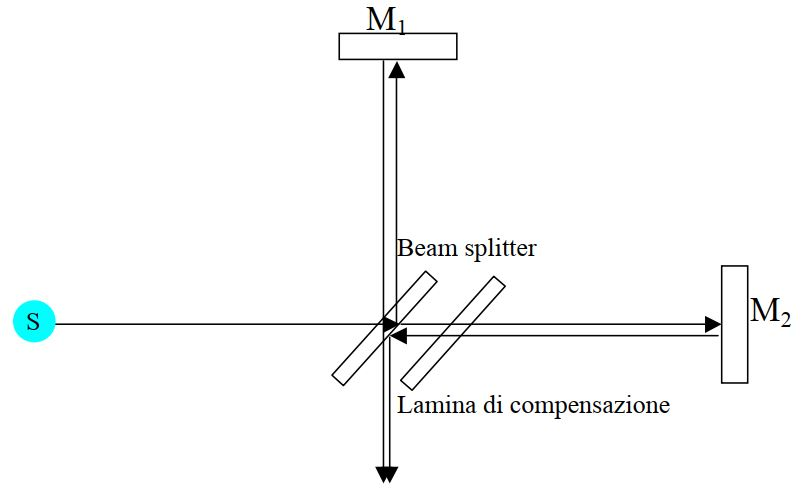
\includegraphics[scale=0.6]{interferometro}
	\caption{Schema dell'interferometro di Michelson}
	\label{fig:int}
\end{figure}
 
 \subsection*{Descrizione dell'interferometro}
 L'interferometro è composto da due bracci di uguale lunghezza al termine dei quali sono posizionati i due specchi M1 ed M2 che riflettono la sorgente, i due segnali andaranno poi a sovrapporsi nel ramo dell'osservatore che potrà visualizzare le frange circolari di interferenza. Lo specchio M2 è orientabile per ottenere il miglior allineamento possibile con l'interferometro, mentre M1 è mobile tramite micrometro che agisce su di una leva meccanica che ne demoltiplica lo spostamento.
 
 \subsection*{Determinazione del fattore di demoltiplica del micrometro}
 In questa parte dell'esperienza è stato utilizzato un laser He-Ne con lunghezza d'onda nota. La prima operazione che si esegue è quella di regolare l'orientamento degli specchi tramite le apposite viti così da centrare la figura di interferenza proiettata su un foglio posto poco distante dallo strumento. A questo punto si esegue la misura vera e propria.\newline
 Il micrometro sul quale si agisce per spostare lo specchio M1 ha una risoluzione di 10$\mu$m. Se lo specchio viene spostato di un tratto $\Delta$X, il cammino ottico varierà di 2$\Delta$X e perciò nella figura di interferenza m, il numero di massimi o minimi che scorrono in un determinato punto, sarà dato da:
\begin{equation*}
2\Delta\mathrm{X} = m\lambda
\end{equation*}
Conoscendo il valore della lunghezza d'onda del laser He-Ne, pari a 632.8 nm, è possibile calcolare il fattore di dempoltiplica del micrometro:
\begin{equation*}
\mathrm{\Delta X = k\Delta S}
\end{equation*}
\begin{equation*}
\mathrm{2k\Delta S = m\lambda} \Rightarrow \mathrm{k = \frac{m\lambda}{2\Delta S}}
\end{equation*}
dove k rappresenta il fattore di demoltiplica e $\Delta$S la misura letta sul micrometro. 
\newpage
\noindent In Tabella~\ref{tab:dem} sono raccolti i dati sul numero di frange osservate, lettura del micrometro e fattore di demoltiplica ottenuto da ciascun membro del gruppo.
\begin{table}[h!]
	\centering
	\caption{Fattore di demoltiplica del micrometro}
	\vspace{1mm}
	\begin{tabular}{ccc}
	\hline
	N° Frange & $\Delta$S & k \\ 
	\hline \hline
	\rem{\dots} & \rem{\dots} & \rem{\dots} \\
	\rem{\dots} & \rem{\dots} & \rem{\dots} \\
	\rem{\dots} & \rem{\dots} & \rem{\dots} \\
	\hline
	\end{tabular}
	\label{tab:dem}
\end{table} 

\noindent Il valore medio del fattore di demoltiplica risulta essere k = \rem{\dots}. Gli errori su k sono stati ottenuti tramite la consueta propagazione con le derivate, come errore su $\Delta$S si è preso un valore inferiore alla risoluzione dello strumento in quanto era individuabile con estrema chiarezza se la misura fosse più vicina ad una tacca o a quella successiva sul micrometro.

\subsection*{Misura della lunghezza d'onda della lampada al mercurio}
In questa fase si sostituisce il laser He-Ne con una lampada al mercurio aspettando qualche minuto che si riscaldi prima di effettuare le osservazioni. Davanti alla lampada viene posto un filtro verde per selezionare una determinata lunghezza d'onda e si pone una punta di riferimento per facilitare la successiva operazione di conteggio delle frange di interferenza. La misura da eseguire è dunque la stessa eseguita per il laser He-Ne, ma ora è useremo il coefficiente di demoltiplica k stimato precedentemente per ottenere la lunghezza d'onda tramite:
\begin{equation*}
\mathrm{\lambda = \frac{2k\Delta S}{m}}
\end{equation*}
Le misurazioni effettuate da ciascun membro del gruppo sono raccolte in Tabella~\ref{tab:hg}.
\begin{table}[h!]
	\centering
	\caption{Lunghezza d'onda della riga verde di Hg}
	\vspace{1mm}
	\begin{tabular}{ccc}
	\hline
	N° Frange & $\Delta$S & $\lambda$ \\ 
	\hline \hline
	\rem{\dots} & \rem{\dots} & \rem{\dots} \\
	\rem{\dots} & \rem{\dots} & \rem{\dots} \\
	\rem{\dots} & \rem{\dots} & \rem{\dots} \\
	\hline
	\end{tabular}
	\label{tab:hg}
\end{table}

\noindent La lunghezza d'onda media risulta essere $\lambda$ = \rem{\dots}. Gli errori sono stati propagati con il metodo delle derivate ed è stata fatta la medisima considerazione fatta in precedenza per l'errore sulla lettura del micrometro.

\subsection*{Osservazione dellle frange di interferenza con la luce bianca}
In questa fase dell'esperienza si vogliono osservare le frange d'interferenza nella luce bianca, cioè non monocromatica. L'effetto in questo caso sarà visibile soltanto quando la differenza dei cammini ottici nei due bracci è dell'ordine della lunghezza d'onda centrale della luce, quindi al massimo qualche micron.

\noindent Al fine di osservare le frange di interferenza è necessario dunque effettuare alcune operazioni preliminari. Si inserisce lo spaziatore di alluminio su uno dei due bracci in modo da rendere i cammini ottici il più simili possibile, si procede dunque a riallineare l'interferometro con la lampada con il filtro ancora in sede per ritrovare le frange, a questo punto si agisce sulla lunghezza del braccio mobile per ottenere la condizione di ugual cammino ottico. Questa condizione sarà verificata osservando la frangia centrale che diventa sempre più grande. A questo punto si rimuove il filtro per osservare le frange d'interferenza nella luce bianca.
 
 
 
 
 
 
 
 
 
 
 
 
 
 
 
 
 
 
 
 
 
 
 
 
 
 
 
 
 
 \end{document}